\documentclass[UTF8]{ctexart}
\usepackage{listings}
\usepackage{booktabs}  
\usepackage{geometry}  
\usepackage{graphicx} 
\usepackage{xcolor}
\usepackage{float}
\usepackage{array}
\usepackage{enumitem}
\usepackage{amsmath,amssymb,bm}
\usepackage[colorlinks=true]{hyperref}
\usepackage[version=4]{mhchem}
\usepackage{siunitx}
\usepackage{tikz}
\usepackage{pgfplots}
\pgfplotsset{compat=1.18}
\graphicspath{{figure/}} % 指定放置图片的子文件夹路径
\geometry{a4paper, left=2.5cm, right=2.5cm, top=2.5cm, bottom=2.5cm}
\definecolor{codegreen}{rgb}{0,0.6,0}
\definecolor{codegray}{rgb}{0.5,0.5,0.5}
\definecolor{codepurple}{rgb}{0.58,0,0.82}
\lstset{
    basicstyle=\ttfamily\footnotesize,
    breaklines=true,
    frame=single,
    numbers=left,
    numberstyle=\tiny\color{codegray},
    keywordstyle=\color{blue},
    commentstyle=\color{codegreen},
    stringstyle=\color{codepurple},
    showstringspaces=false
}


\begin{document}
\title{计算流体力学期末大作业}
\author{朱林-2200011028}
\date{\today}
\maketitle

\section{数理算法原理}
\subsection{问题描述}
\subsubsection{物理情形}
Sod激波管问题是一个一维理想气体流动问题:无限长管道中,初始时刻($t=0$)在$x=0$处有一薄膜分隔两侧气体:
\begin{itemize}
    \item 左侧($x<0$): 高压区,状态为$(\rho_L, u_L, p_L)$
    \item 右侧($x>0$): 低压区,状态为$(\rho_R, u_R, p_R)$
\end{itemize}

薄膜在$t=0^+$时刻瞬时破裂,两侧气体开始相互作用,产生复杂的波系结构。

\subsubsection{标准初始条件}
采用以下无量纲初始条件:
\begin{align*}
\text{左侧:} & \quad \rho_L = 1.0,  u_L = 0.0,  p_L = 1.0 \\
\text{右侧:} & \quad \rho_R = 0.125,  u_R = 0.0,  p_R = 0.1
\end{align*}

\subsection{控制方程}
流动由一维欧拉方程描述:
\begin{align}
&\frac{\partial \mathbf{U}}{\partial t} + \frac{\partial f(\mathbf{U})}{\partial x} = 0 \\
&\mathbf{U} = \begin{bmatrix} \rho \\ \rho u \\ E \end{bmatrix}, \quad
f(\mathbf{U}) = \begin{bmatrix} \rho u \\ \rho u^2 + p \\ u(E + p) \end{bmatrix}
\end{align}
其中总能密度$E = \rho e = \rho (C_v T + \frac{1}{2}u^2)$。

\subsection{Riemann问题精确解}
通过查阅资料,Sod激波管问题的精确解可以通过黎曼问题的解法得到。该问题的解由四个区域组成,分别对应不同的流动状态和波系结构。

\subsubsection{波系结构}
薄膜破裂后,将产生以下三种波结构:
\begin{enumerate}
    \item \textbf{膨胀波(稀疏波)}:向左传播进入高压区($x<0$)
    \item \textbf{接触间断}:向右传播的分界面,分隔原始左右侧气体
    \item \textbf{激波}:向右传播进入低压区($x>0$)
\end{enumerate}

这些波将流场划分为四个特征区域(如图\ref{fig:wave_structure}所示):
\begin{itemize}
    \item \textbf{区域1} ($x < x_{\text{left}}$):未扰动的左侧高压区,保持初始状态 $(\rho_L, u_L, p_L)$
    \item \textbf{区域2} ($x_{\text{left}} < x < x_{\text{contact}}$):膨胀波后均匀区,状态为 $(\rho_2, u^*, p^*)$
    \item \textbf{区域3} ($x_{\text{contact}} < x < x_{\text{shock}}$):接触间断与激波间均匀区,状态为 $(\rho_3, u^*, p^*)$
    \item \textbf{区域4} ($x > x_{\text{shock}}$):未扰动的右侧低压区,保持初始状态 $(\rho_R, u_R, p_R)$
\end{itemize}

其中 $u^*$ 和 $p^*$ 为接触间断处的速度和压力,各波位置随时间线性变化:
$$x_{\text{left}} = -c_L t, \quad x_{\text{contact}} = u^* t, \quad x_{\text{shock}} = W_s t$$
$W_s$ 为激波传播速度,$c_L = \sqrt{\gamma p_L/\rho_L}$ 为左侧声速。

\begin{figure}[H]
    \centering
    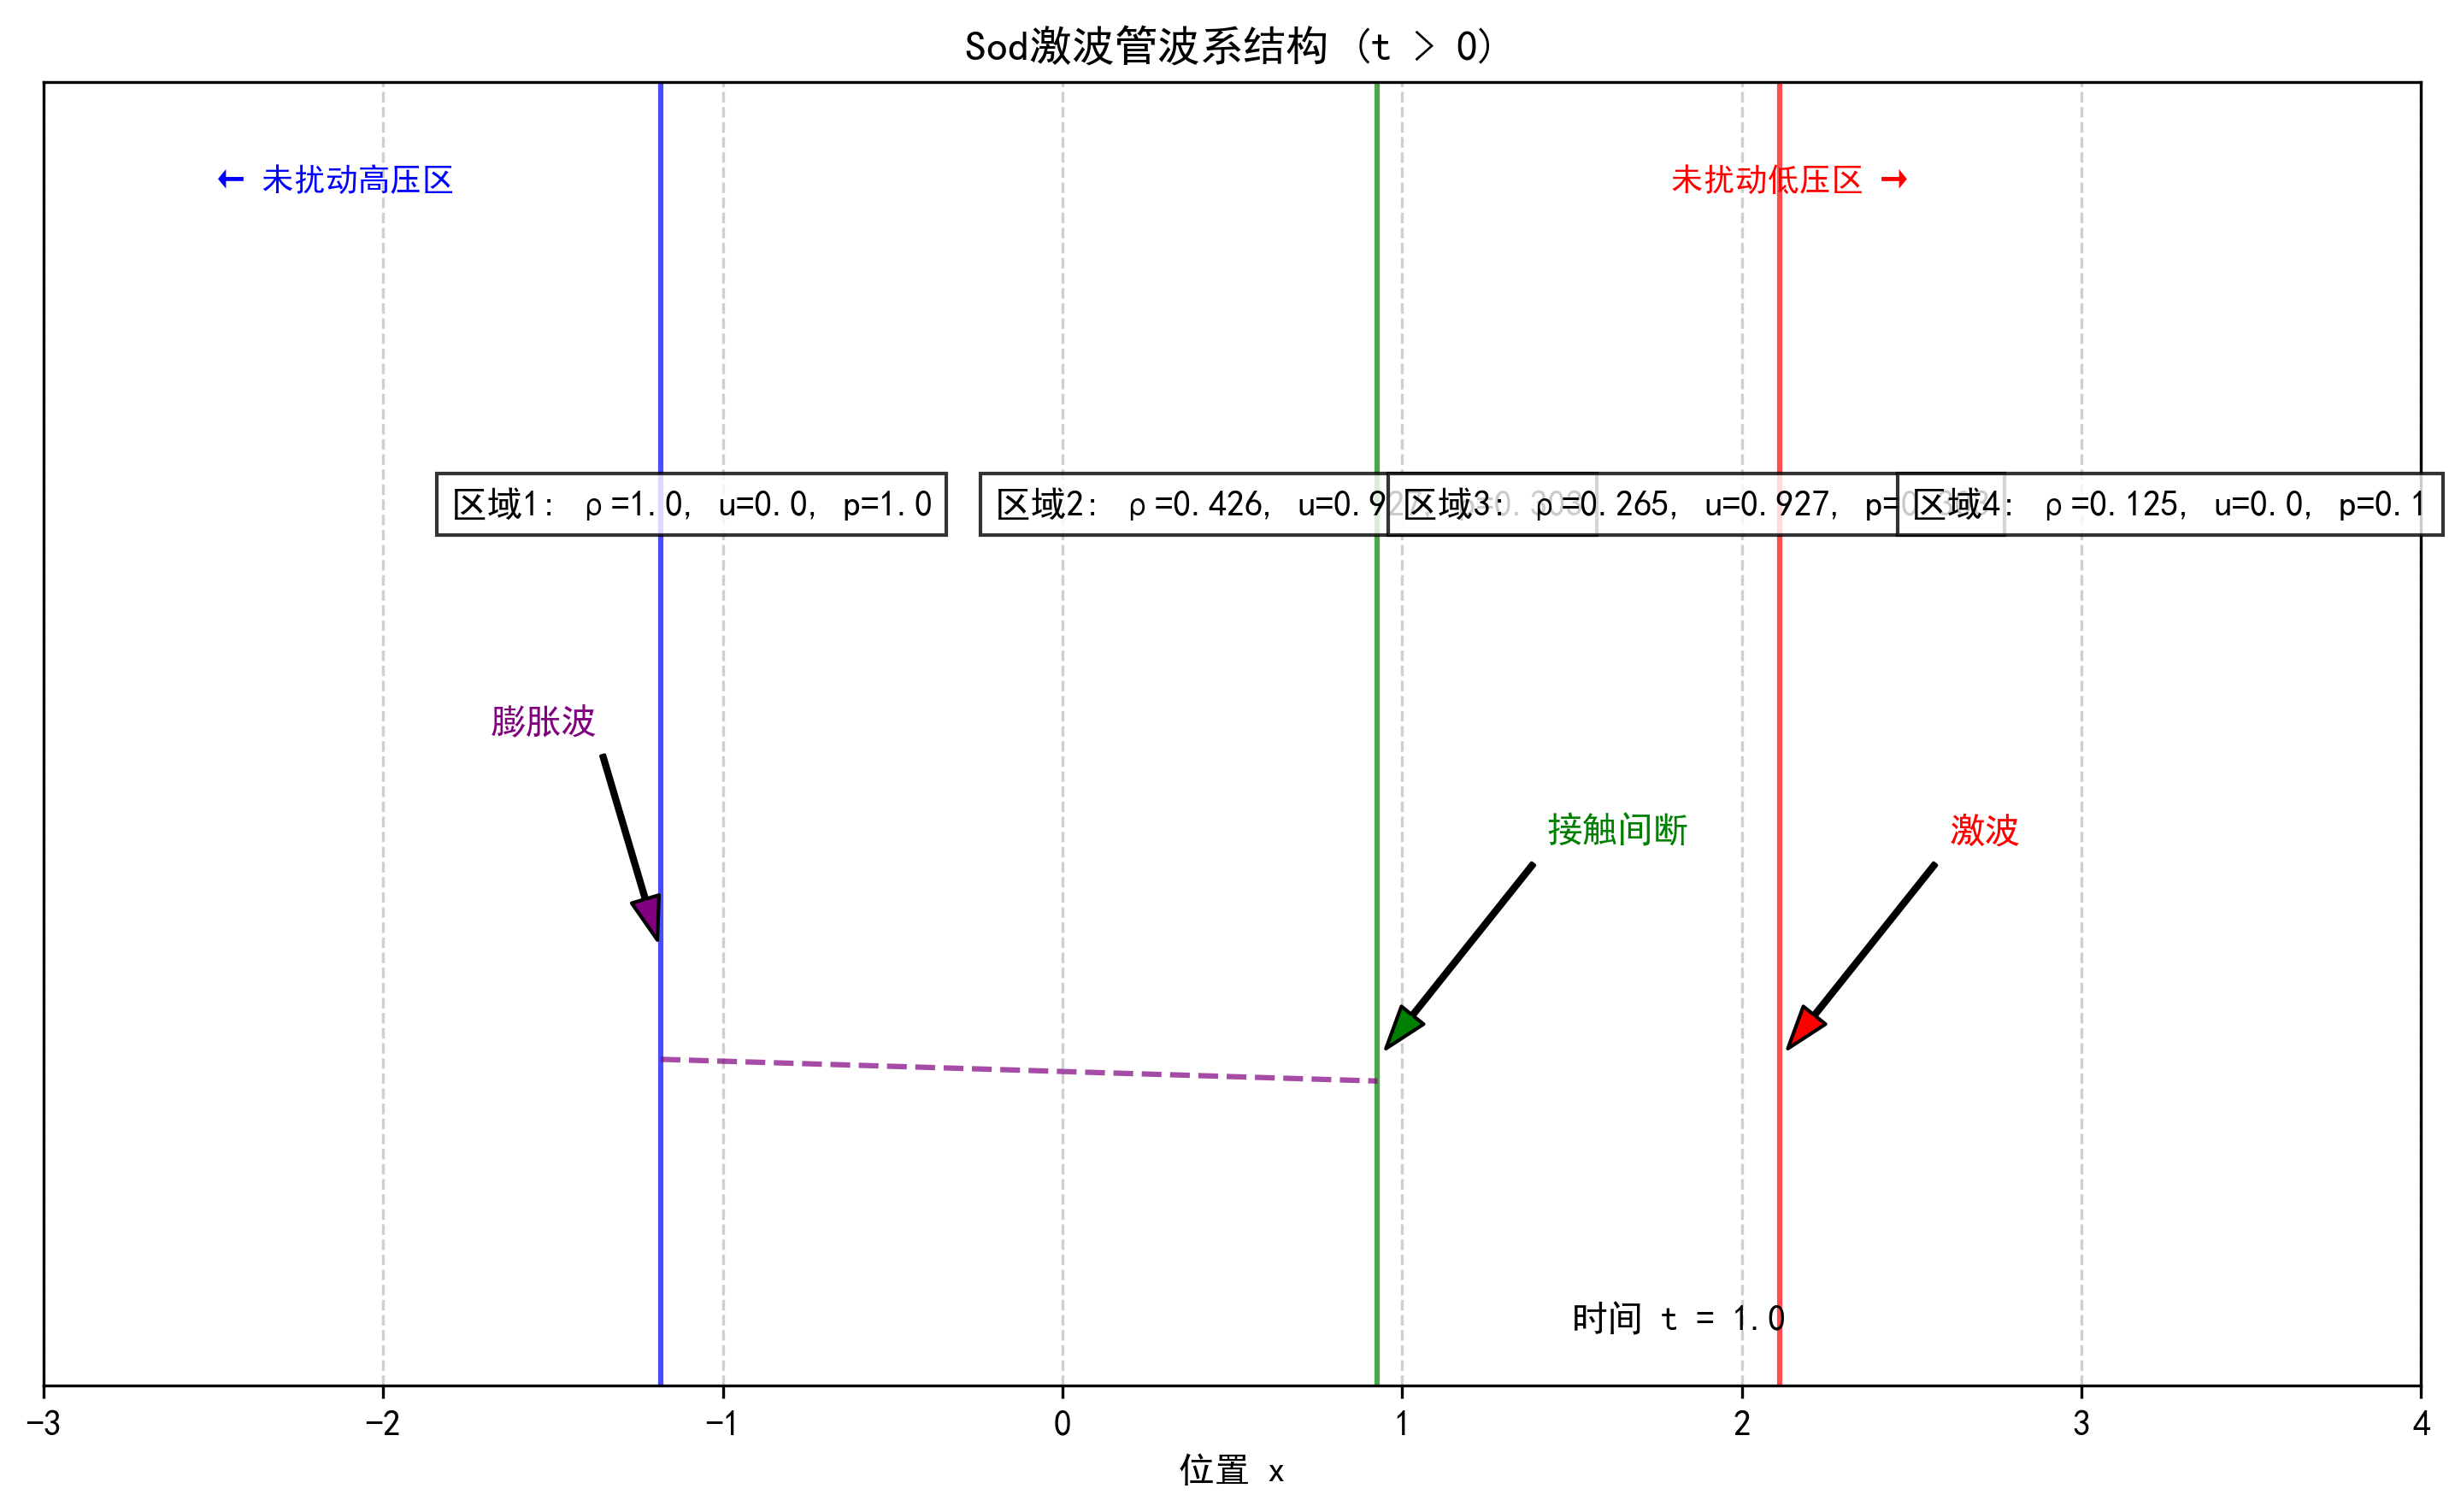
\includegraphics[width=0.8\textwidth]{wave_structure.png}
    \caption{Sod激波管典型波系结构(t>0)}
    \label{fig:wave_structure}
\end{figure}

\subsubsection{解析解表达式}
解析解通过求解以下方程组获得:

1. \textbf{膨胀波区(稀疏波,$x/t \in [-c_L, u^*-c_2]$)}  
   等熵流动关系:
   \begin{align*}
   u &= \frac{2}{\gamma+1}\left(c_L + \frac{x}{t}\right) \\
   c &= c_L - \frac{\gamma-1}{2}u \\
   \rho &= \rho_L \left(\frac{c}{c_L}\right)^{2/(\gamma-1)} \\
   p &= p_L \left(\frac{c}{c_L}\right)^{2\gamma/(\gamma-1)}
   \end{align*}

2. \textbf{接触间断条件}($x = u^* t$)  
   压力与速度连续:
   $$p_2 = p_3 = p^*, \quad u_2 = u_3 = u^*$$

3. \textbf{激波关系}(Rankine-Hugoniot条件)  
   \begin{align*}
   \frac{\rho_3}{\rho_R} &= \frac{(\gamma+1)p^* + (\gamma-1)p_R}{(\gamma-1)p^* + (\gamma+1)p_R} \\
   u^* &= u_R + \frac{c_R}{\gamma}\left(\frac{p^*}{p_R}-1\right)\sqrt{\frac{2\gamma}{(\gamma+1)p^*/p_R + (\gamma-1)}}
   \end{align*}

4. \textbf{膨胀波与接触间断衔接}  
   $$u^* = u_L + \frac{2c_L}{\gamma-1}\left[1 - \left(\frac{p^*}{p_L}\right)^{(\gamma-1)/(2\gamma)}\right]$$

其中 $\gamma$ 为比热比(空气取1.4)。通过数值求解上述非线性方程组可得 $p^*$ 和 $u^*$,进而确定全场解。

作为黎曼问题的最简单形式,Sod激波管是理解更复杂流动机理的基础,同时常用于计算流体中作为典型案例检验算法和格式。


%附录
\newpage
\appendix
\section{AI工具使用声明表}
\begin{table}[H]
    \centering
    \begin{tabular}{c|c|c}
        \hline
        使用内容 & 工具名称 & 使用目的 \\ \hline
        hw2.tex 1-9行、图片插入 & Github Copilot & 调整pdf格式,调用宏包,省略插入图片的重复性工作 \\ 
        main.py 6-15行 & DeepSeek & 修正 matplotlib 中文显示问题 \\ 
        ReadMe.md框架 & DeepSeek & 在DeepSeek的帮助下生成一个框架,在此基础上增加而来 \\
        .gitignore & Github Copilot & 针对于python和latex的.gitignore文件,完全由Copilot生成  
    \end{tabular}
    \label{tab:AI_tools}
\end{table}
\end{document}